\documentclass[twoside,a4wide,12pt]{article}\usepackage[]{graphicx}\usepackage[]{color}
%% maxwidth is the original width if it is less than linewidth
%% otherwise use linewidth (to make sure the graphics do not exceed the margin)
\makeatletter
\def\maxwidth{ %
  \ifdim\Gin@nat@width>\linewidth
    \linewidth
  \else
    \Gin@nat@width
  \fi
}
\makeatother

\definecolor{fgcolor}{rgb}{0.345, 0.345, 0.345}
\newcommand{\hlnum}[1]{\textcolor[rgb]{0.686,0.059,0.569}{#1}}%
\newcommand{\hlstr}[1]{\textcolor[rgb]{0.192,0.494,0.8}{#1}}%
\newcommand{\hlcom}[1]{\textcolor[rgb]{0.678,0.584,0.686}{\textit{#1}}}%
\newcommand{\hlopt}[1]{\textcolor[rgb]{0,0,0}{#1}}%
\newcommand{\hlstd}[1]{\textcolor[rgb]{0.345,0.345,0.345}{#1}}%
\newcommand{\hlkwa}[1]{\textcolor[rgb]{0.161,0.373,0.58}{\textbf{#1}}}%
\newcommand{\hlkwb}[1]{\textcolor[rgb]{0.69,0.353,0.396}{#1}}%
\newcommand{\hlkwc}[1]{\textcolor[rgb]{0.333,0.667,0.333}{#1}}%
\newcommand{\hlkwd}[1]{\textcolor[rgb]{0.737,0.353,0.396}{\textbf{#1}}}%

\usepackage{framed}
\makeatletter
\newenvironment{kframe}{%
 \def\at@end@of@kframe{}%
 \ifinner\ifhmode%
  \def\at@end@of@kframe{\end{minipage}}%
  \begin{minipage}{\columnwidth}%
 \fi\fi%
 \def\FrameCommand##1{\hskip\@totalleftmargin \hskip-\fboxsep
 \colorbox{shadecolor}{##1}\hskip-\fboxsep
     % There is no \\@totalrightmargin, so:
     \hskip-\linewidth \hskip-\@totalleftmargin \hskip\columnwidth}%
 \MakeFramed {\advance\hsize-\width
   \@totalleftmargin\z@ \linewidth\hsize
   \@setminipage}}%
 {\par\unskip\endMakeFramed%
 \at@end@of@kframe}
\makeatother

\definecolor{shadecolor}{rgb}{.97, .97, .97}
\definecolor{messagecolor}{rgb}{0, 0, 0}
\definecolor{warningcolor}{rgb}{1, 0, 1}
\definecolor{errorcolor}{rgb}{1, 0, 0}
\newenvironment{knitrout}{}{} % an empty environment to be redefined in TeX

\usepackage{alltt}
%\DefineVerbatimEnvironment{Sinput}{Verbatim} {xleftmargin=2em,frame=single}
%\DefineVerbatimEnvironment{Soutput}{Verbatim} {xleftmargin=2em,frame=single}
\usepackage[left=2.5cm,top=2cm,right=2cm,bottom=2.5cm,bindingoffset=0.5cm]{geometry}
\usepackage{amsmath} 
\usepackage[affil-it]{authblk}
\usepackage{hyperref}
\usepackage{fullpage}
\usepackage{pdflscape}
\usepackage[backend=bibtex,sorting=none,style=ieee]{biblatex}
\usepackage{setspace}
\bibliography{biblio}


\title{Proteochemometrics (PCM) with 'camb'\\
{\bf C}hemistry {\bf A}ware {\bf M}odel {\bf B}uilder\\
Cambridge. November 2013}

\author[1,3]{\rm Isidro Cortes-Ciriano\thanks{isidrolauscher@gmail.com}} 
\author[2,3]{\rm Daniel Murrell\thanks{dsmurrell@gmail.com}}
\affil[1]{Unite de Bioinformatique Structurale, Institut Pasteur and CNRS UMR 3825, Structural Biology and Chemistry Department, 25-28, rue Dr. Roux, 75 724 Paris, France.}
\affil[2]{Unilever Centre for Molecular Science Informatics, Department of Chemistry, University of Cambridge, Cambridge, United Kingdom.}
\affil[*]{Equal contributors}

\setlength{\parindent}{0pt}
\IfFileExists{upquote.sty}{\usepackage{upquote}}{}

\begin{document}

\maketitle
\onehalfspacing






\maketitle

Firstly, we load the package and set the working directory:
\begin{knitrout}
\definecolor{shadecolor}{rgb}{0.969, 0.969, 0.969}\color{fgcolor}\begin{kframe}
\begin{alltt}
\hlkwd{library}\hlstd{(camb)}
\hlkwd{setwd}\hlstd{(}\hlstr{"/Users/icortes/Desktop/camb_final/camb/examples/COX"}\hlstd{)}
\end{alltt}
\end{kframe}
\end{knitrout}

\section{Compounds}

\subsection{Reading and Preprocessing}
\begin{knitrout}
\definecolor{shadecolor}{rgb}{0.969, 0.969, 0.969}\color{fgcolor}\begin{kframe}
\begin{alltt}
\hlstd{smiles} \hlkwb{<-} \hlkwd{read.table}\hlstd{(}\hlstr{"smiles_COX.smi"}\hlstd{,} \hlkwc{header} \hlstd{=} \hlnum{FALSE}\hlstd{,}
    \hlkwc{comment.char} \hlstd{=} \hlkwd{c}\hlstd{(}\hlstr{""}\hlstd{))}
\end{alltt}
\end{kframe}
\end{knitrout}

Given that some smiles contain smarts patterns where the hash symbol is present, we need to avoid switch of the argumment comment.char in order not to clip the smiles:

\begin{knitrout}
\definecolor{shadecolor}{rgb}{0.969, 0.969, 0.969}\color{fgcolor}\begin{kframe}
\begin{alltt}
\hlkwd{StandardiseMolecules}\hlstd{(}\hlkwc{structures.file}\hlstd{=}\hlstr{"smiles_COX.smi"}\hlstd{,}
\hlkwc{standardised.file}\hlstd{=}\hlstr{"standardised.sdf"}\hlstd{,}
\hlkwc{removed.file}\hlstd{=}\hlstr{"removed.sdf"}\hlstd{,}
\hlkwc{output}\hlstd{=}\hlstr{"standardisation_COX_info.csv"}\hlstd{,}
\hlkwc{remove.inorganic}\hlstd{=}\hlnum{TRUE}\hlstd{,}
\hlkwc{fluorine.limit}\hlstd{=}\hlopt{-}\hlnum{1}\hlstd{,}
\hlkwc{chlorine.limit}\hlstd{=}\hlopt{-}\hlnum{1}\hlstd{,}
\hlkwc{bromine.limit}\hlstd{=}\hlopt{-}\hlnum{1}\hlstd{,}
\hlkwc{iodine.limit}\hlstd{=}\hlopt{-}\hlnum{1}\hlstd{,}
\hlkwc{min.mass.limit}\hlstd{=}\hlnum{20}\hlstd{,} \hlcom{#suggested value 20}
\hlkwc{max.mass.limit}\hlstd{=}\hlnum{900}\hlstd{)}\hlcom{#suggested value  900)}
\end{alltt}
\end{kframe}
\end{knitrout}

The properties of all molecules and the index (in the column 'kept') indicating which molecules were deleted are written to a file called standardisation\_COX\_info.csv.

\begin{knitrout}
\definecolor{shadecolor}{rgb}{0.969, 0.969, 0.969}\color{fgcolor}\begin{kframe}
\begin{alltt}
\hlstd{standardised_info} \hlkwb{<-} \hlkwd{read.table}\hlstd{(}\hlstr{"standardisation_COX_info.csv"}\hlstd{,}
    \hlkwc{header} \hlstd{=} \hlnum{TRUE}\hlstd{,} \hlkwc{sep} \hlstd{=} \hlstr{","}\hlstd{)}
\hlkwd{head}\hlstd{(standardised_info)}
\end{alltt}
\end{kframe}
\end{knitrout}


In this case, the criteria we chose to remove compounds (the arguments of the StandardiseMolecules function) were not really stringent, so all molecules were kept. This can be seen in the kept field, given that for all compounds (rows) we have a 1.\\
Similarly, the properties of a .sdf file can be accessed witn the function:
\begin{knitrout}
\definecolor{shadecolor}{rgb}{0.969, 0.969, 0.969}\color{fgcolor}\begin{kframe}
\begin{alltt}
\hlkwd{ShowPropertiesSDF}\hlstd{(}\hlstr{"standardised.sdf"}\hlstd{,} \hlkwc{type} \hlstd{=} \hlnum{1}\hlstd{)}
\end{alltt}
\end{kframe}
\end{knitrout}

A given property can be accessed, or all of them. In the latter case, a data.frame with all properties is returned:
\begin{knitrout}
\definecolor{shadecolor}{rgb}{0.969, 0.969, 0.969}\color{fgcolor}\begin{kframe}
\begin{alltt}
\hlstd{logS} \hlkwb{<-} \hlkwd{GetPropertySDF}\hlstd{(}\hlstr{"standardised.sdf"}\hlstd{,} \hlkwc{property} \hlstd{=} \hlstr{"logS"}\hlstd{,}
    \hlkwc{number_processed} \hlstd{=} \hlnum{10}\hlstd{,} \hlkwc{type} \hlstd{=} \hlnum{1}\hlstd{)}
\end{alltt}


{\ttfamily\noindent\bfseries\color{errorcolor}{\#\# Error: line 2 did not have 11 elements}}\begin{alltt}
\hlstd{all_properties} \hlkwb{<-} \hlkwd{GetPropertiesSDF}\hlstd{(}\hlstr{"standardised.sdf"}\hlstd{,} \hlkwc{number_processed} \hlstd{=} \hlnum{10}\hlstd{,}
    \hlkwc{type} \hlstd{=} \hlnum{1}\hlstd{)}
\end{alltt}


{\ttfamily\noindent\bfseries\color{errorcolor}{\#\# Error: no lines available in input}}\begin{alltt}
\hlkwd{head}\hlstd{(all_properties)}
\end{alltt}


{\ttfamily\noindent\bfseries\color{errorcolor}{\#\# Error: error in evaluating the argument 'x' in selecting a method for function 'head': Error: object 'all\_properties' not found}}\end{kframe}
\end{knitrout}


\subsection{PaDEL Descriptors}
\begin{knitrout}
\definecolor{shadecolor}{rgb}{0.969, 0.969, 0.969}\color{fgcolor}\begin{kframe}
\begin{alltt}
\hlstd{descriptors_COX} \hlkwb{<-} \hlkwd{GeneratePadelDescriptors}\hlstd{(}\hlkwc{standardised.file} \hlstd{=} \hlstr{"smiles_COX.smi"}\hlstd{,}
    \hlkwc{threads} \hlstd{=} \hlnum{1}\hlstd{)}
\hlstd{descriptors} \hlkwb{<-} \hlkwd{RemoveStandardisedPrefix}\hlstd{(descriptors)}
\hlkwd{saveRDS}\hlstd{(descriptors,} \hlkwc{file} \hlstd{=} \hlstr{"descriptors.rds"}\hlstd{)}
\hlstd{descriptors} \hlkwb{<-} \hlkwd{readRDS}\hlstd{(}\hlstr{"descriptors.rds"}\hlstd{)}
\end{alltt}
\end{kframe}
\end{knitrout}


Sometimes, some descriptors are not calcualted for all molecules, thus giving a 'NA' or 'Inf' as descriptor values. Instead of removing that descriptor for all molecules, the missing descriptor values can be {\it imputed} from the corresponding descriptor values of the rest of molecules. To do that, 'Inf' values are converted to 'NA', and then imputed:

\begin{knitrout}
\definecolor{shadecolor}{rgb}{0.969, 0.969, 0.969}\color{fgcolor}\begin{kframe}
\begin{alltt}
\hlstd{descriptors} \hlkwb{<-} \hlkwd{ReplaceInfinitesWithNA}\hlstd{(descriptors)}
\hlstd{descriptors} \hlkwb{<-} \hlkwd{ImputeFeatures}\hlstd{(descriptors)}
\end{alltt}
\end{kframe}
\end{knitrout}


\subsection{Circular Morgan Fingerprints}
\begin{knitrout}
\definecolor{shadecolor}{rgb}{0.969, 0.969, 0.969}\color{fgcolor}\begin{kframe}
\begin{alltt}
\hlkwd{Sys.setenv}\hlstd{(}\hlkwc{RDBASE} \hlstd{=} \hlstr{"/usr/local/share/RDKit"}\hlstd{)}
\hlkwd{Sys.setenv}\hlstd{(}\hlkwc{PYTHONPATH} \hlstd{=} \hlstr{"/usr/local/lib/python2.7/site-packages"}\hlstd{)}
\hlstd{fps_COX_512} \hlkwb{<-} \hlkwd{MorganFPs}\hlstd{(}\hlkwc{bits} \hlstd{=} \hlnum{512}\hlstd{,} \hlkwc{radius} \hlstd{=} \hlnum{2}\hlstd{,} \hlkwc{type} \hlstd{=} \hlstr{"smi"}\hlstd{,}
    \hlkwc{mols} \hlstd{=} \hlstr{"smiles_COX.smi"}\hlstd{,} \hlkwc{output} \hlstd{=} \hlstr{"COX"}\hlstd{,} \hlkwc{keep} \hlstd{=} \hlstr{"hashed_counts"}\hlstd{)}
\hlkwd{saveRDS}\hlstd{(fps_COX_512,} \hlkwc{file} \hlstd{=} \hlstr{"fps_COX_512.rds"}\hlstd{)}
\hlstd{fps_COX_512} \hlkwb{<-} \hlkwd{readRDS}\hlstd{(}\hlstr{"fps_COX_512.rds"}\hlstd{)}
\end{alltt}
\end{kframe}
\end{knitrout}


\section{Targets}

\subsection{Read and Preprocessing}
We read the read the amino acids from a .csv file:
\begin{knitrout}
\definecolor{shadecolor}{rgb}{0.969, 0.969, 0.969}\color{fgcolor}\begin{kframe}
\begin{alltt}
\hlstd{amino_accompound_compound_IDs} \hlkwb{<-} \hlkwd{read.table}\hlstd{(}\hlstr{"AAs_COX.csv"}\hlstd{,}
    \hlkwc{sep} \hlstd{=} \hlstr{","}\hlstd{,} \hlkwc{header} \hlstd{=} \hlnum{TRUE}\hlstd{,} \hlkwc{colClasses} \hlstd{=} \hlkwd{c}\hlstd{(}\hlstr{"character"}\hlstd{),}
    \hlkwc{row.names} \hlstd{=} \hlnum{1}\hlstd{)}
\hlstd{amino_accompound_IDs} \hlkwb{<-} \hlstd{amino_accompound_IDs[,} \hlnum{2}\hlopt{:}\hlkwd{ncol}\hlstd{(amino_accompound_IDs)]}
\end{alltt}
\end{kframe}
\end{knitrout}


\begin{knitrout}
\definecolor{shadecolor}{rgb}{0.969, 0.969, 0.969}\color{fgcolor}\begin{kframe}
\begin{alltt}
\hlstd{amino_accompound_IDs_zscales} \hlkwb{<-} \hlkwd{AA_descs}\hlstd{(}\hlkwc{Data} \hlstd{= amino_accompound_IDs,}
    \hlkwc{type} \hlstd{=} \hlstr{"Z3"}\hlstd{)}
\end{alltt}
\end{kframe}
\end{knitrout}


Ensuingly, we save the descriptors in a .rds file.
\begin{knitrout}
\definecolor{shadecolor}{rgb}{0.969, 0.969, 0.969}\color{fgcolor}\begin{kframe}
\begin{alltt}
\hlcom{# saveRDS(amino_accompound_IDs_zscales,file='Z3_COX.rds')}
\hlstd{amino_accompound_IDs_zscales} \hlkwb{<-} \hlkwd{readRDS}\hlstd{(}\hlstr{"Z3_COX.rds"}\hlstd{)}
\end{alltt}
\end{kframe}
\end{knitrout}


In the case that we needed whole sequence descriptors, they can be calculated with the function 'SeqDescs'. The functin takes as argument either a UniProt identifier, or a \{matrix, dataframe\} with the protein sequences. If a UniProt identifier is provided, the function gets firstly the sequence and then calculates the descriptors on the sequence.

\begin{knitrout}
\definecolor{shadecolor}{rgb}{0.969, 0.969, 0.969}\color{fgcolor}\begin{kframe}
\begin{alltt}
\hlstd{Seq_descriptors_P00374} \hlkwb{<-} \hlkwd{SeqDescs}\hlstd{(}\hlstr{"P00374"}\hlstd{,} \hlkwc{UniProtID} \hlstd{=} \hlnum{TRUE}\hlstd{,}
    \hlkwc{type} \hlstd{=} \hlkwd{c}\hlstd{(}\hlstr{"AAC"}\hlstd{,} \hlstr{"DC"}\hlstd{))}
\end{alltt}
\end{kframe}
\end{knitrout}

The available types of descriptor are:\cite{protr}
- Amino Acid Composition ("AAC")\\
- Dipeptide Composition ("DC")\\
- Tripeptide Composition ("TC")\\
- Normalized Moreau-Broto Autocorrelation ("MoreauBroto")\\
- Moran Autocorrelation ("Moran")\\
- Geary Autocorrelation ("Geary")\\
- CTD (Composition/Transition/Distribution) ("CTD")\\
- Conjoint Traid ("CTriad")\\
- Sequence Order Coupling Number ("SOCN")\\
- Quasi-sequence Order Descriptors ("QSO")\\
- Pseudo Amino Acid Composition ("PACC")\\
- Amphiphilic Pseudo Amino Acid Composition ("APAAC")\\

\begin{knitrout}
\definecolor{shadecolor}{rgb}{0.969, 0.969, 0.969}\color{fgcolor}\begin{kframe}
\begin{alltt}
\hlstd{Seq_descriptors_P00374} \hlkwb{<-} \hlkwd{SeqDescs}\hlstd{(}\hlstr{"P00374"}\hlstd{)}
\hlstd{Seq_descriptors_P00374}
\end{alltt}
\begin{verbatim}
##              A       R       N       D        C       E
## P00374 0.02674 0.04278 0.05348 0.04813 0.005348 0.08556
##              Q       G       H       I      L       K
## P00374 0.03743 0.06952 0.01604 0.04813 0.1016 0.09091
##              M       F       P       S       T       W
## P00374 0.03743 0.04813 0.06417 0.06417 0.03743 0.01604
##              Y       V
## P00374 0.03209 0.07487
\end{verbatim}
\end{kframe}
\end{knitrout}


\subsection{Reading the Data-set Information}
Now, we are going to read the file with the information about the dataset, namely: target names, bioctivities, etc..
Be careful: when reading smiles from a .csv file into an R dataframe, the smils are clipped after a hash ('\#') symbol.
Good practice: also keep the smiles alone in a \{.smi,.smiles\} file.

\begin{knitrout}
\definecolor{shadecolor}{rgb}{0.969, 0.969, 0.969}\color{fgcolor}\begin{kframe}
\begin{alltt}
\hlstd{dataset} \hlkwb{<-} \hlkwd{readRDS}\hlstd{(}\hlstr{"COX_dataset_info.rds"}\hlstd{)}
\hlstd{bioactivity} \hlkwb{<-} \hlstd{dataset}\hlopt{$}\hlstd{standard_value}
\end{alltt}
\end{kframe}
\end{knitrout}

The bioactivity is in nM. We convert it to pIC50:
\begin{knitrout}
\definecolor{shadecolor}{rgb}{0.969, 0.969, 0.969}\color{fgcolor}\begin{kframe}
\begin{alltt}
\hlstd{bioactivity} \hlkwb{<-} \hlstd{bioactivity} \hlopt{*} \hlnum{10}\hlopt{^-}\hlnum{9}
\hlstd{bioactivity} \hlkwb{<-} \hlopt{-}\hlkwd{log}\hlstd{(bioactivity,} \hlkwc{base} \hlstd{=} \hlnum{10}\hlstd{)}
\end{alltt}
\end{kframe}
\end{knitrout}


\section{Data-set Visualization}
Compounds can be depicted with the function 'PlotMolecules'. It returns a list of four plots, and plots can also be written into a .pdf file.
\begin{knitrout}
\definecolor{shadecolor}{rgb}{0.969, 0.969, 0.969}\color{fgcolor}\begin{kframe}
\begin{alltt}
\hlstd{plot_molecules} \hlkwb{<-} \hlkwd{PlotMolecules}\hlstd{(}\hlstr{"standardised.sdf"}\hlstd{,}
    \hlkwc{IDs} \hlstd{=} \hlkwd{c}\hlstd{(}\hlnum{1}\hlstd{,} \hlnum{2}\hlstd{,} \hlnum{3}\hlstd{,} \hlnum{4}\hlstd{),} \hlkwc{pdf.file} \hlstd{=} \hlstr{"test_comp_visualization.pdf"}\hlstd{,}
    \hlkwc{useNameAsTitle} \hlstd{=} \hlnum{TRUE}\hlstd{,} \hlkwc{PDFMain} \hlstd{=} \hlkwa{NULL}\hlstd{)}
\end{alltt}
\begin{verbatim}
## [1] 1
## [1] 2
## [1] 3
## [1] 4
\end{verbatim}
\begin{alltt}
\hlstd{plot_molecules[[}\hlnum{1}\hlstd{]]}
\end{alltt}
\end{kframe}\begin{figure}[]


{\centering 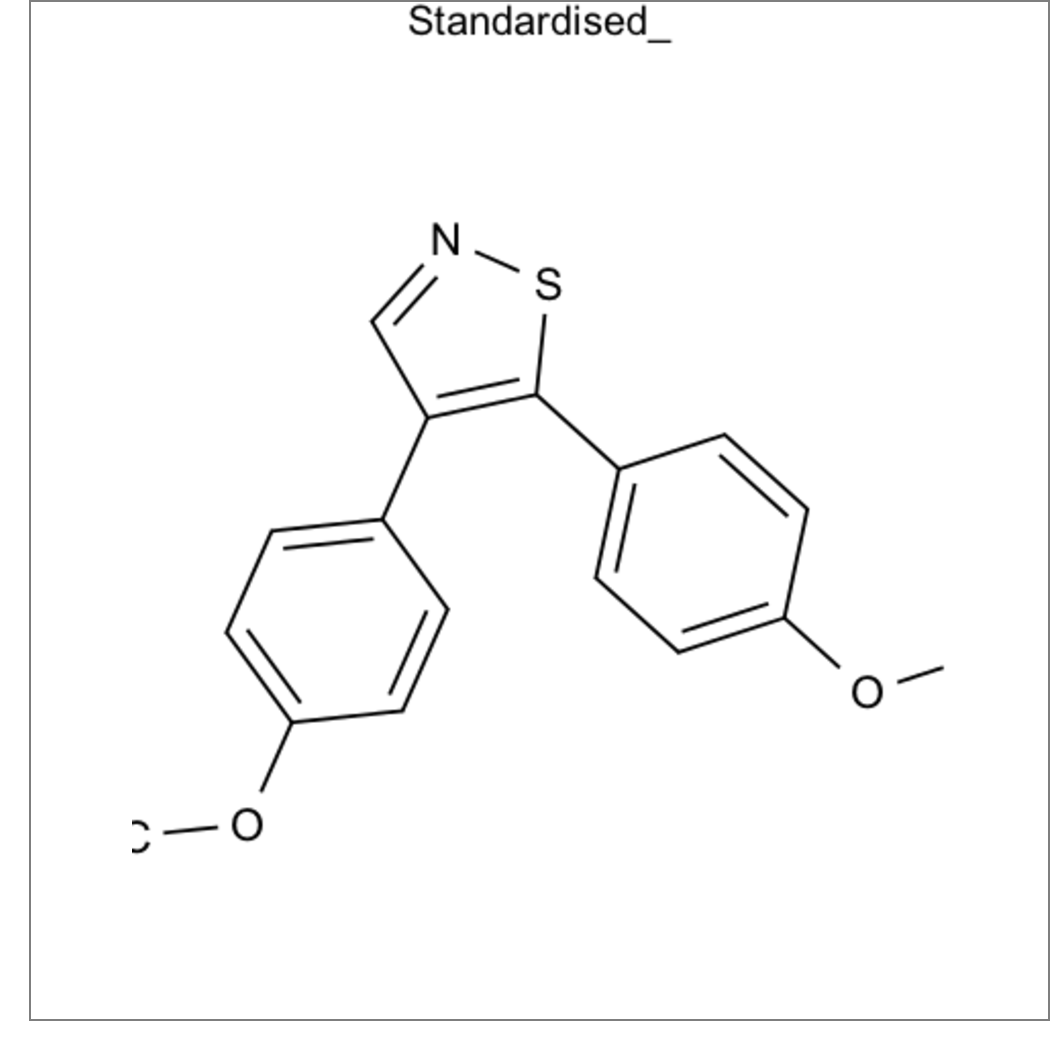
\includegraphics[width=12cm]{figure/unnamed-chunk-19} 

}

\caption[Example of compoud depiction]{Example of compoud depiction.\label{fig:unnamed-chunk-19}}
\end{figure}


\end{knitrout}


We can have a look at the response variable:
\begin{knitrout}
\definecolor{shadecolor}{rgb}{0.969, 0.969, 0.969}\color{fgcolor}\begin{kframe}
\begin{alltt}
\hlstd{dens_resp} \hlkwb{<-} \hlkwd{DensityResponse}\hlstd{(bioactivity,} \hlkwc{xlab} \hlstd{=} \hlstr{"pIC50"}\hlstd{,}
    \hlkwc{main} \hlstd{=} \hlstr{""}\hlstd{,} \hlkwc{ylab} \hlstd{=} \hlstr{"Densitiy"}\hlstd{,} \hlkwc{TitleSize} \hlstd{=} \hlnum{26}\hlstd{,} \hlkwc{XAxisSize} \hlstd{=} \hlnum{20}\hlstd{,}
    \hlkwc{YAxisSize} \hlstd{=} \hlnum{20}\hlstd{,} \hlkwc{TitleAxesSize} \hlstd{=} \hlnum{24}\hlstd{,} \hlkwc{AngleLab} \hlstd{=} \hlnum{0}\hlstd{,}
    \hlkwc{lmar} \hlstd{=} \hlnum{0}\hlstd{,} \hlkwc{rmar} \hlstd{=} \hlnum{0}\hlstd{,} \hlkwc{bmar} \hlstd{=} \hlnum{0}\hlstd{,} \hlkwc{tmar} \hlstd{=} \hlnum{0}\hlstd{)}
\end{alltt}
\end{kframe}
\end{knitrout}


Plotting a PCA analysis of the target descriptors gives:
\begin{knitrout}
\definecolor{shadecolor}{rgb}{0.969, 0.969, 0.969}\color{fgcolor}\begin{kframe}
\begin{alltt}
\hlstd{target_PCA} \hlkwb{<-} \hlkwd{PCAProt}\hlstd{(amino_accompound_IDs_zscales,}
    \hlkwc{SeqsName} \hlstd{= dataset}\hlopt{$}\hlstd{accession)}
\hlstd{plot_PCA_Cox} \hlkwb{<-} \hlkwd{PCAProtPlot}\hlstd{(target_PCA,} \hlkwc{PointSize} \hlstd{=} \hlnum{8}\hlstd{,}
    \hlkwc{main} \hlstd{=} \hlstr{""}\hlstd{,} \hlkwc{TitleSize} \hlstd{=} \hlnum{26}\hlstd{,} \hlkwc{XAxisSize} \hlstd{=} \hlnum{20}\hlstd{,} \hlkwc{YAxisSize} \hlstd{=} \hlnum{20}\hlstd{,}
    \hlkwc{TitleAxesSize} \hlstd{=} \hlnum{24}\hlstd{,} \hlkwc{LegendPosition} \hlstd{=} \hlstr{"bottom"}\hlstd{,}
    \hlkwc{RowLegend} \hlstd{=} \hlnum{2}\hlstd{,} \hlkwc{ColLegend} \hlstd{=} \hlnum{6}\hlstd{,} \hlkwc{LegendTitleSize} \hlstd{=} \hlnum{10}\hlstd{,}
    \hlkwc{LegendTextSize} \hlstd{=} \hlnum{10}\hlstd{)}
\end{alltt}
\begin{verbatim}
## [1] "Sequence names provided in the third column of the data.frame"
\end{verbatim}
\begin{alltt}
\hlstd{plot_PCA_Cox}
\end{alltt}
\end{kframe}\begin{figure}[]


{\centering 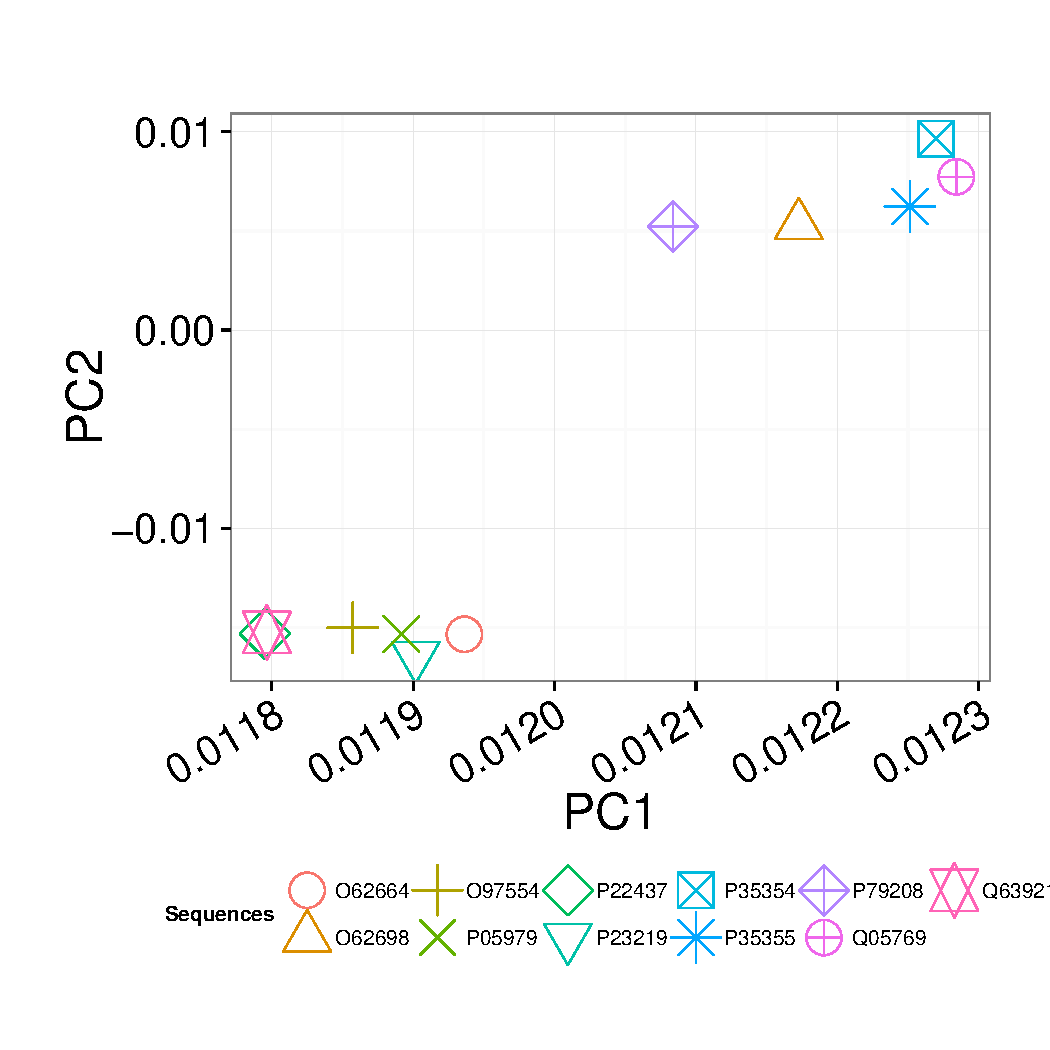
\includegraphics[width=\maxwidth]{figure/unnamed-chunk-21} 

}

\caption[PCA Analysis on the
Amino Acid Descriptors]{PCA Analysis on the
Amino Acid Descriptors\label{fig:unnamed-chunk-21}}
\end{figure}


\end{knitrout}


Similarly, we can analyze the chemical space by calculating pairwise compound similarities based upon the compound descriptors. In this case, we use the Jaccard metric to calculate the distance between compounds.
\begin{knitrout}
\definecolor{shadecolor}{rgb}{0.969, 0.969, 0.969}\color{fgcolor}\begin{kframe}
\begin{alltt}
\hlcom{# pw_dist_comp_fps <-}
\hlcom{# PairwiseDist(fps_COX_512,method='jaccard')}
\hlcom{# saveRDS(pw_dist_comp_fps,file='pairwise_dist_COX.rds')}
\hlstd{pw_dist_comp_fps} \hlkwb{<-} \hlkwd{readRDS}\hlstd{(}\hlstr{"pairwise_dist_COX.rds"}\hlstd{)}
\hlstd{plot_pwd} \hlkwb{<-} \hlkwd{PairwiseDistPlot}\hlstd{(pw_dist_comp_fps,} \hlkwc{xlab} \hlstd{=} \hlstr{"Jaccard Similarity"}\hlstd{,}
    \hlkwc{ylab} \hlstd{=} \hlstr{"Density"}\hlstd{,} \hlkwc{TitleSize} \hlstd{=} \hlnum{26}\hlstd{,} \hlkwc{XAxisSize} \hlstd{=} \hlnum{20}\hlstd{,}
    \hlkwc{YAxisSize} \hlstd{=} \hlnum{20}\hlstd{,} \hlkwc{TitleAxesSize} \hlstd{=} \hlnum{24}\hlstd{,} \hlkwc{lmar} \hlstd{=} \hlnum{0}\hlstd{,} \hlkwc{rmar} \hlstd{=} \hlnum{0}\hlstd{,}
    \hlkwc{bmar} \hlstd{=} \hlnum{0}\hlstd{,} \hlkwc{tmar} \hlstd{=} \hlnum{0}\hlstd{)}
\end{alltt}
\end{kframe}
\end{knitrout}


\begin{knitrout}
\definecolor{shadecolor}{rgb}{0.969, 0.969, 0.969}\color{fgcolor}\begin{kframe}
\begin{alltt}
\hlkwd{library}\hlstd{(ggplot2)}
\hlkwd{grid.arrange}\hlstd{(dens_resp, plot_pwd,} \hlkwc{nrow} \hlstd{=} \hlnum{2}\hlstd{)}
\end{alltt}
\end{kframe}\begin{figure}[]


{\centering 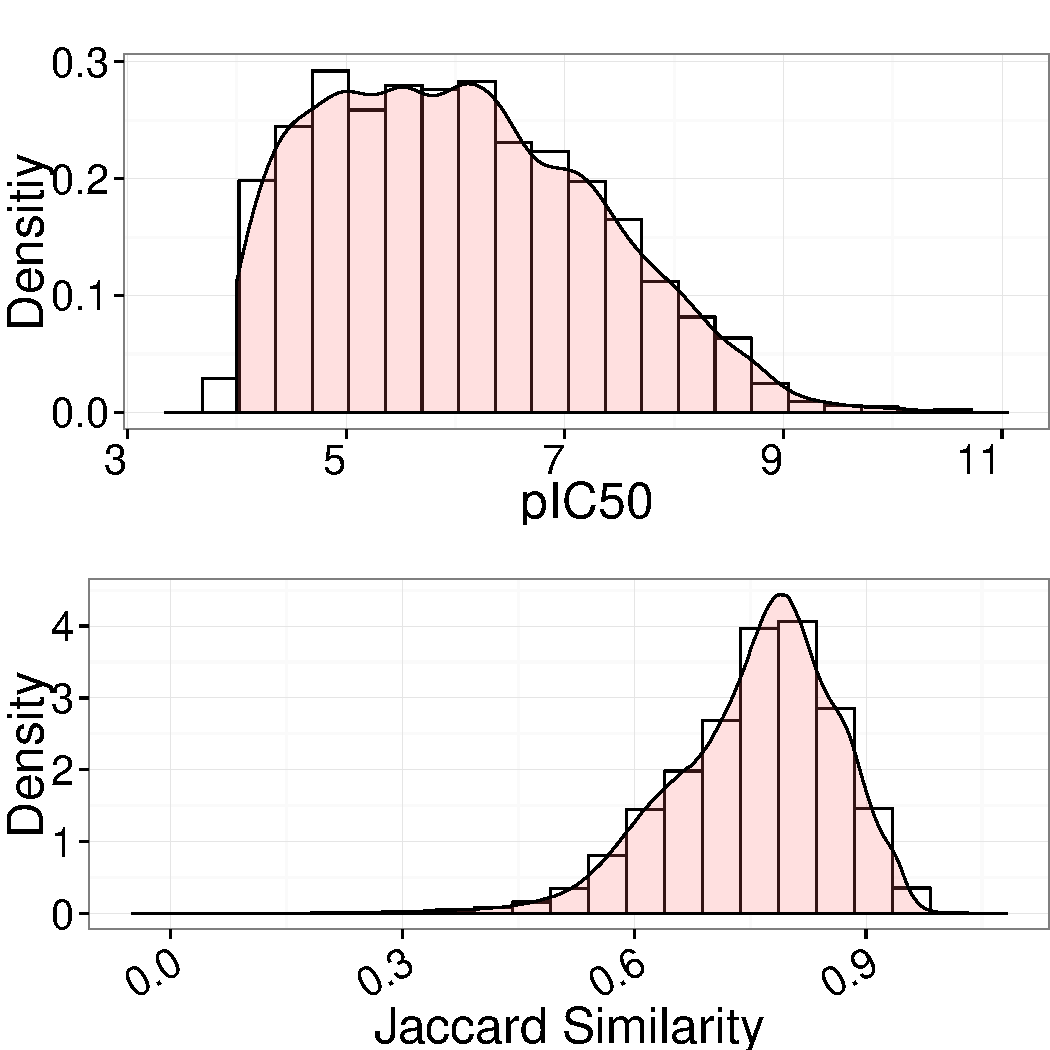
\includegraphics[width=\maxwidth]{figure/unnamed-chunk-23} 

}

\caption[Density of the response variable (left)]{Density of the response variable (left). Pairwise Compound Jaccard Similarity (right)\label{fig:unnamed-chunk-23}}
\end{figure}


\end{knitrout}


%\newpage
Before any modeling attempt, it is interesting to know which is the maximum performance achievable {\it on the basis} of the available data.\\ 
By that, we consider the experimental uncertainty and the size of our data-set. 
In this case, a Gaussian Process (GP) model was trained in Matlab (data not shown) where the experimental uncertainty was optimized as a hyperparameter. The obtained value was 0.60.\\
This value is in accordance with recently prublished value of 0.68 for public IC50 data.
With the function 'MaxPerf', we can calculate the manximum achievable performance:

\begin{knitrout}
\definecolor{shadecolor}{rgb}{0.969, 0.969, 0.969}\color{fgcolor}\begin{kframe}
\begin{alltt}
\hlstd{max_performance} \hlkwb{<-} \hlkwd{MaxPerf}\hlstd{(}\hlkwc{meanNoise} \hlstd{=} \hlnum{0}\hlstd{,} \hlkwc{sdNoise} \hlstd{=} \hlnum{0.6}\hlstd{,}
    \hlkwc{meanResp} \hlstd{=} \hlkwd{mean}\hlstd{(bioactivity),} \hlkwc{sdResp} \hlstd{=} \hlkwd{sd}\hlstd{(bioactivity),}
    \hlkwc{lenPred} \hlstd{=} \hlnum{800}\hlstd{)}
\end{alltt}
\end{kframe}
\end{knitrout}


The function returns a list of four plots. By using the function 'plotGrid' we can create a grid of plots in the following way:

\begin{knitrout}
\definecolor{shadecolor}{rgb}{0.969, 0.969, 0.969}\color{fgcolor}\begin{kframe}
\begin{alltt}
\hlkwd{plotGrid}\hlstd{(}\hlkwc{plots} \hlstd{=} \hlkwd{c}\hlstd{(max_performance}\hlopt{$}\hlstd{p1, max_performance}\hlopt{$}\hlstd{p2,}
    \hlstd{max_performance}\hlopt{$}\hlstd{p3, max_performance}\hlopt{$}\hlstd{p4))}
\end{alltt}
\end{kframe}
\end{knitrout}


\section{Statistical Pre-processing}
Bioactivity annotations in ChEMBL are sometimes redundant, meaning that for a given target-compound combination there are more than one annotated values.\\
To avoid this issue, we will remove redundant pairs and will keep the mean bioactivity value for those compound-target combinations repeated.\\
%To do that, we run the file \"remove_duplicates.R\":
\begin{knitrout}
\definecolor{shadecolor}{rgb}{0.969, 0.969, 0.969}\color{fgcolor}\begin{kframe}
\begin{alltt}
\hlkwd{source}\hlstd{(}\hlstr{"remove_duplicates.R"}\hlstd{)}
\end{alltt}
\end{kframe}
\end{knitrout}


Now, we load the dataset without repetitions generated in the previous step. In addition, we remove those columns not containing descriptors (e.g. compound name):
\begin{knitrout}
\definecolor{shadecolor}{rgb}{0.969, 0.969, 0.969}\color{fgcolor}\begin{kframe}
\begin{alltt}
\hlstd{dataset} \hlkwb{<-} \hlkwd{readRDS}\hlstd{(}\hlstr{"Whole_dataset_NO_REP.rds"}\hlstd{)}
\hlstd{killset} \hlkwb{<-} \hlkwd{expression}\hlstd{(}\hlkwd{c}\hlstd{(tid, pref_name, accession,}
    \hlstd{organism, chembl_id, standard_value, standard_units,}
    \hlstd{standard_type, chembl_id.1, Name, Name.1, Name.2,}
    \hlstd{rows))}
\hlstd{bioactivity} \hlkwb{<-} \hlstd{dataset}\hlopt{$}\hlstd{standard_value}
\hlstd{compound_IDs} \hlkwb{<-} \hlstd{dataset}\hlopt{$}\hlstd{chembl_id.1}
\hlstd{dataset} \hlkwb{<-} \hlkwd{subset}\hlstd{(dataset,} \hlkwc{select} \hlstd{=} \hlopt{-}\hlkwd{eval}\hlstd{(killset))}
\end{alltt}
\end{kframe}
\end{knitrout}


Subsequently, we split the dataset into a training (70\%) and a hold-out (external; 30\%) set that will be used to assess the predictive ability of the models. Furthermore, we remove the following descriptors: (i) those with a variance close to zero (near-zero variance), and (ii) those highly correlated:
\begin{knitrout}
\definecolor{shadecolor}{rgb}{0.969, 0.969, 0.969}\color{fgcolor}\begin{kframe}
\begin{alltt}
\hlcom{# split the dataset into a training and holdout set}
\hlstd{dataset} \hlkwb{<-} \hlkwd{SplitSet}\hlstd{(compound_IDs, dataset, bioactivity,}
    \hlkwc{percentage} \hlstd{=} \hlnum{30}\hlstd{)}

\hlcom{# remove the descriptors that are highly correlated}
\hlcom{# or have low variance}
\hlstd{dataset} \hlkwb{<-} \hlkwd{RemoveNearZeroVarianceFeatures}\hlstd{(dataset,}
    \hlkwc{frequencyCutoff} \hlstd{=} \hlnum{30}\hlopt{/}\hlnum{1}\hlstd{)}
\hlstd{dataset} \hlkwb{<-} \hlkwd{RemoveHighlyCorrelatedFeatures}\hlstd{(dataset)}
\end{alltt}
\end{kframe}
\end{knitrout}


We convert the descriptors to z-scores by centering them to zero mean and scaling their values to unit variance:
\begin{knitrout}
\definecolor{shadecolor}{rgb}{0.969, 0.969, 0.969}\color{fgcolor}\begin{kframe}
\begin{alltt}
\hlstd{dataset} \hlkwb{<-} \hlkwd{PreProcess}\hlstd{(dataset)}
\end{alltt}
\end{kframe}
\end{knitrout}


Given that cross-validation (CV) will be used to optimize the hyperparameters of the models, we divide the training setin 5 folds:
\begin{knitrout}
\definecolor{shadecolor}{rgb}{0.969, 0.969, 0.969}\color{fgcolor}\begin{kframe}
\begin{alltt}
\hlstd{dataset} \hlkwb{<-} \hlkwd{GetCVTrainControl}\hlstd{(dataset)}
\hlkwd{saveRDS}\hlstd{(dataset,} \hlkwc{file} \hlstd{=} \hlstr{"dataset_COX_preprocessed.rda"}\hlstd{)}
\end{alltt}
\end{kframe}
\end{knitrout}


\section{Model Training}

\begin{knitrout}
\definecolor{shadecolor}{rgb}{0.969, 0.969, 0.969}\color{fgcolor}\begin{kframe}
\begin{alltt}
\hlstd{dataset} \hlkwb{<-} \hlkwd{readRDS}\hlstd{(}\hlstr{"dataset_COX_preprocessed.rda"}\hlstd{)}
\hlcom{# Set the number of cores for parallelization of}
\hlcom{# the training}
\hlkwd{library}\hlstd{(doMC)}
\end{alltt}


{\ttfamily\noindent\itshape\color{messagecolor}{\#\# Loading required package: iterators}}\begin{alltt}
\hlkwd{registerDoMC}\hlstd{(}\hlkwc{cores} \hlstd{=} \hlnum{4}\hlstd{)}  \hlcom{#from the package 'doMC'}
\end{alltt}
\end{kframe}
\end{knitrout}


\subsection{Support Vector Machines (SVM)}
Firstly, a SVM will be trained. We define an exponential grid (base 2) to optimize the hyperparameters:

\begin{knitrout}
\definecolor{shadecolor}{rgb}{0.969, 0.969, 0.969}\color{fgcolor}\begin{kframe}
\begin{alltt}
\hlstd{method} \hlkwb{<-} \hlstr{"svmRadial"}
\hlstd{exp_grid} \hlkwb{<-} \hlkwd{expGrid}\hlstd{(}\hlkwc{power.from} \hlstd{=} \hlopt{-}\hlnum{8}\hlstd{,} \hlkwc{power.to} \hlstd{=} \hlopt{-}\hlnum{6}\hlstd{,}
    \hlkwc{power.by} \hlstd{=} \hlnum{2}\hlstd{,} \hlkwc{base} \hlstd{=} \hlnum{2}\hlstd{)}
\hlstd{tune.grid} \hlkwb{<-} \hlkwd{expand.grid}\hlstd{(}\hlkwc{.sigma} \hlstd{= exp_grid)}
\end{alltt}
\end{kframe}
\end{knitrout}


Training:
\begin{knitrout}
\definecolor{shadecolor}{rgb}{0.969, 0.969, 0.969}\color{fgcolor}\begin{kframe}
\begin{alltt}
\hlcom{# modelCoxSVMrad <- train(dataset$x.train,}
\hlcom{# dataset$y.train, method, tuneGrid=tune.grid,}
\hlcom{# trControl=dataset$trControl)}
\hlcom{# saveRDS(modelCoxSVMrad, file='svm_model_COX.rds')}
\hlstd{modelCoxSVMrad} \hlkwb{<-} \hlkwd{readRDS}\hlstd{(}\hlstr{"COXsvm.rds"}\hlstd{)}
\end{alltt}
\end{kframe}
\end{knitrout}


\subsection{Random Forest}
We proceed similarly in the case of a random forest model.

\begin{knitrout}
\definecolor{shadecolor}{rgb}{0.969, 0.969, 0.969}\color{fgcolor}\begin{kframe}
\begin{alltt}
\hlstd{method} \hlkwb{<-} \hlstr{"rf"}
\hlstd{tune.grid} \hlkwb{<-} \hlkwd{expand.grid}\hlstd{(}\hlkwc{.mtry} \hlstd{=} \hlkwd{seq}\hlstd{(}\hlnum{5}\hlstd{,} \hlnum{100}\hlstd{,} \hlnum{5}\hlstd{))}

\hlcom{# modelCoxRF<- train(dataset$x.train,}
\hlcom{# dataset$y.train, method, tuneGrid=tune.grid,}
\hlcom{# trControl=dataset$trControl) saveRDS(modelCoxRF,}
\hlcom{# file='rf_model_COX.rds')}
\hlstd{modelCoxRF} \hlkwb{<-} \hlkwd{readRDS}\hlstd{(}\hlstr{"COXrf.rds"}\hlstd{)}
\end{alltt}
\end{kframe}
\end{knitrout}


\section{Model Evaluation}

Once the models are trained, the cross validated metrics can be calculated:

\begin{knitrout}
\definecolor{shadecolor}{rgb}{0.969, 0.969, 0.969}\color{fgcolor}\begin{kframe}
\begin{alltt}
\hlcom{# Cross Validation Metrics.  We assume the metric}
\hlcom{# used for the choice of the best combination of}
\hlcom{# hyperparameters is 'RMSE'.  This can be checked}
\hlcom{# by: 'my_model'$metric}
\hlstd{RMSE_CV} \hlkwb{=} \hlkwd{signif}\hlstd{(}\hlkwd{min}\hlstd{(}\hlkwd{as.vector}\hlstd{(}\hlkwd{na.omit}\hlstd{(modelCoxRF}\hlopt{$}\hlstd{results}\hlopt{$}\hlstd{RMSE))),}
    \hlkwc{digits} \hlstd{=} \hlnum{3}\hlstd{)}
\hlstd{Rsquared_CV} \hlkwb{=} \hlstd{modelCoxRF}\hlopt{$}\hlstd{results}\hlopt{$}\hlstd{Rsquared[}\hlkwd{which}\hlstd{(modelCoxRF}\hlopt{$}\hlstd{results}\hlopt{$}\hlstd{RMSE} \hlopt
    \hlkwd{min}\hlstd{(modelCoxRF}\hlopt{$}\hlstd{results}\hlopt{$}\hlstd{RMSE,} \hlkwc{na.rm} \hlstd{=} \hlnum{TRUE}\hlstd{))]}
\hlkwd{print}\hlstd{(RMSE_CV)}
\end{alltt}
\begin{verbatim}
## [1] 0.78
\end{verbatim}
\begin{alltt}
\hlkwd{print}\hlstd{(Rsquared_CV)}
\end{alltt}
\begin{verbatim}
## [1] 0.5834
\end{verbatim}
\end{kframe}
\end{knitrout}


On the basis of the soundness of the obtained models, we predict the values for the hod-out set:
\begin{knitrout}
\definecolor{shadecolor}{rgb}{0.969, 0.969, 0.969}\color{fgcolor}\begin{kframe}
\begin{alltt}
\hlstd{holdout.predictions} \hlkwb{<-} \hlkwd{as.vector}\hlstd{(}\hlkwd{predict}\hlstd{(modelCoxRF,}
    \hlkwc{newdata} \hlstd{= dataset}\hlopt{$}\hlstd{x.holdout))}
\end{alltt}
\end{kframe}
\end{knitrout}


We evaluate the predictive ability of our models by calculation the following statistical metrics:\\

{\bf Internal validation:}
\\
\begin{equation}
q_{{\it int}}^{2} = 1 - \frac {\sum_{i=1}^{N} (y_{i} - \widetilde{y}_{i})^{2}} {\sum_{i=1}^{N} (y_{i} - \bar{y}_{tr})^{2}}
\end{equation}
% cross-validated correlation coefficient

\begin{equation}
RMSE_{int} = \frac {\sqrt {(y_i - \widetilde{y}_i)^{2}}} {N}
\end{equation}

where $N$, $y_i$, $\widetilde{y}_i$ and $\bar{y}_{tr}$ represent the size of the training set, the observed, the predicted and the averaged values of the response variable for those datapoints included in the training set. The {\it i}th position within the training set is defined by {\it i}.  
\\
\\
{\bf External validation:}
\\

\begin{equation}
q_{{\it ext}}^{2} = 1 - \frac {\sum_{j=1}^{N} (y_j-\widetilde{y}_j)^{2}}  {\sum_{j=1}^{N} (y_j - \bar{y}_{ext})^{2}}
\end{equation}

\begin{equation}
RMSE_{ext} = \frac {\sqrt {(y_i - \widetilde{y}_i)^{2}}} {N} 
\end{equation}

\begin{equation}
R_{ext}^{2} = \frac {{\sum_{i=1}^{N} (y_{i} - \bar{y}_{ext})}  (\widetilde{y}_{i} - \overset{-}{\widetilde{y}_{ext}})} 
{\sqrt{\sum_{i=1}^{N} (y_{i} - \bar{y}_{ext})^{2} \sum{ (\widetilde{y}_{i} - \overset{-}{\widetilde{y}_{ext}})^{2}}}}
\end{equation}

\begin{equation}
R_{0\:ext}^2 = 1 - \frac {\sum_{j=1}^{N} (y_{j} - \widetilde{y}_{j}^{ r0})^{2}} {\sum_{j=1}^{N} (y_{j} - \bar{y}_{ext})^{2}} 
\end{equation}

where $N$, $y_j$, $\widetilde{y}_j$, $\bar{y}_{ext}$ and $\breve{y}_j$ represent the size of the training set, the observed, the predicted, the averaged values and the fitted
values of the response variable for those datapoints comprising the external set. The {\it j}th position within the external set is defined by {\it j}. $R_{0\:ext}^2$ is the square of the coefficient of determination through the origin, being $\widetilde{y}_{j}^{ r0} = k \widetilde{y}_j$ the regression through the origin (observed versus predicted) and $k$ its slope.\\
For a detailed discussion of both the evaluation of the predictive ability through the external set and different formulations for $q^{2}$, see ref.\cite{consonni}. 
To be considered as predictive, a model must satisfy the following criteria:\cite{beware,earnest}
\\
\begin{enumerate}
\item $q_{{\it int}}^{2} > 0.5$
\item $R_{ext}^2 > 0.6$
\item $ \frac {(R_{ext}^2 - R_{0\:ext}^2)} {R_{ext}^2} < 0.1$
\item $0.85 \leq k \leq 1.15$
\end{enumerate}

The metrics for the external validatin are given by:
\begin{knitrout}
\definecolor{shadecolor}{rgb}{0.969, 0.969, 0.969}\color{fgcolor}\begin{kframe}
\begin{alltt}
\hlstd{MetricsRf} \hlkwb{<-} \hlkwd{Validation}\hlstd{(holdout.predictions, dataset}\hlopt{$}\hlstd{y.holdout)}
\hlstd{MetricsRf}
\end{alltt}
\begin{verbatim}
## $R2
## [1] 0.6073
## 
## $R02
## [1] 0.602
## 
## $Q2
## [1] 0.5998
## 
## $RMSE
## [1] 0.7675
## 
## $Slope
## [1] 0.9906
## 
## $MAE
## [1] 0.5851
\end{verbatim}
\end{kframe}
\end{knitrout}


To have a look at the correlation between predicted and observed values, we can use the 'CorrelationPlot' function:

\begin{knitrout}
\definecolor{shadecolor}{rgb}{0.969, 0.969, 0.969}\color{fgcolor}\begin{kframe}
\begin{alltt}
\hlkwd{CorrelationPlot}\hlstd{(}\hlkwc{pred} \hlstd{= holdout.predictions,} \hlkwc{obs} \hlstd{= dataset}\hlopt{$}\hlstd{y.holdout,}
    \hlkwc{PointSize} \hlstd{=} \hlnum{3}\hlstd{,} \hlkwc{ColMargin} \hlstd{=} \hlstr{"blue"}\hlstd{,} \hlkwc{TitleSize} \hlstd{=} \hlnum{26}\hlstd{,}
    \hlkwc{XAxisSize} \hlstd{=} \hlnum{20}\hlstd{,} \hlkwc{YAxisSize} \hlstd{=} \hlnum{20}\hlstd{,} \hlkwc{TitleAxesSize} \hlstd{=} \hlnum{24}\hlstd{,}
    \hlkwc{margin} \hlstd{=} \hlnum{2}\hlstd{,} \hlkwc{PointColor} \hlstd{=} \hlstr{"black"}\hlstd{,} \hlkwc{PointShape} \hlstd{=} \hlnum{16}\hlstd{,}
    \hlkwc{MarginWidth} \hlstd{=} \hlnum{1.5}\hlstd{)}
\end{alltt}
\end{kframe}\begin{figure}[]


{\centering 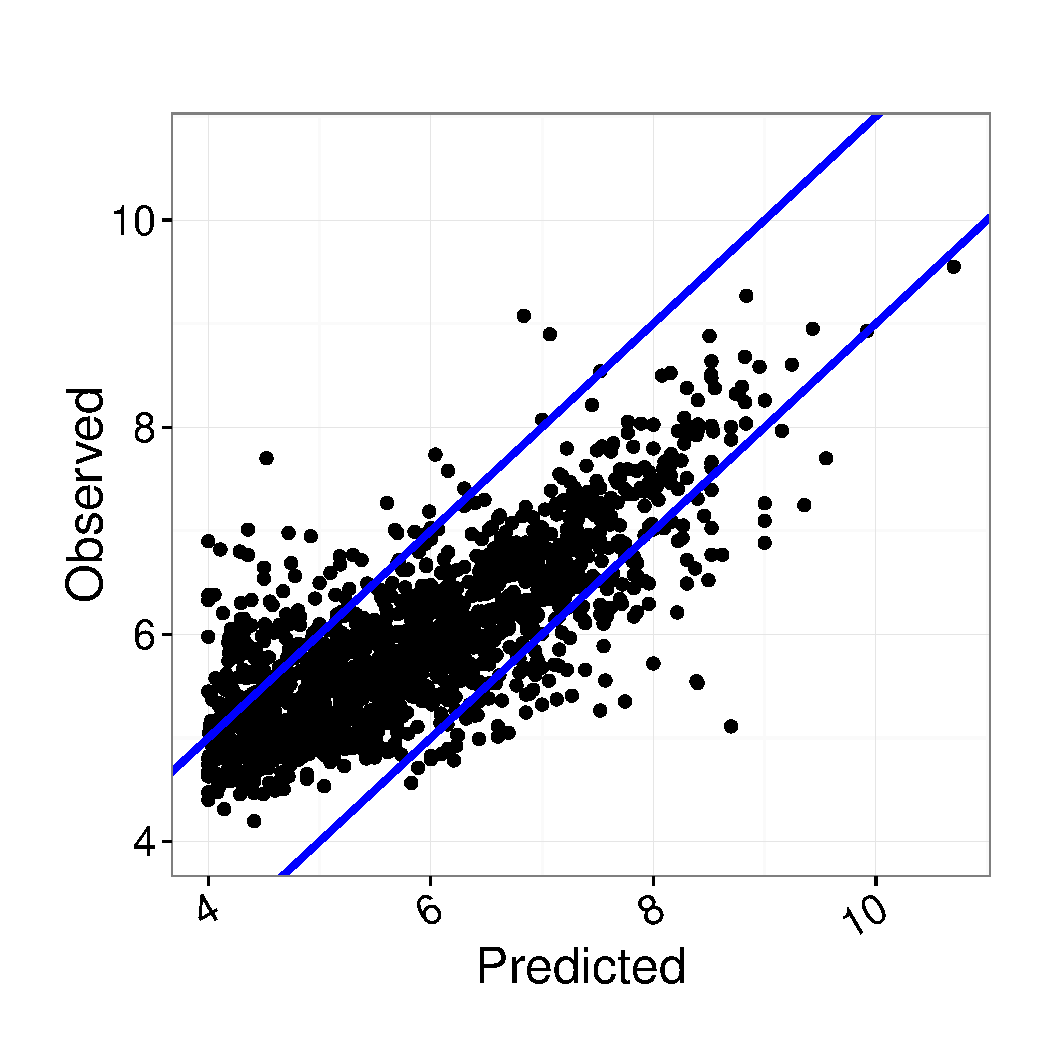
\includegraphics[width=\maxwidth]{figure/unnamed-chunk-38} 

}

\caption[Predicted vs Observed]{Predicted vs Observed\label{fig:unnamed-chunk-38}}
\end{figure}


\end{knitrout}


%\section{Bibliography}
\newpage
\printbibliography

\end{document}
